\subsection{Land Usage}

To gain a comprehensive understanding of land usage patterns and their impact on urban dynamics, we analyze different land usage at four increasingly larger scales. This is achieved by calculating the median land usage area of each region in the city, with the median being computed using progressively larger kernels. By examining land usage at multiple scales, we can uncover patterns that might not be apparent at a single scale, providing deeper insights into the relationship between land use and various urban phenomena, such as crime rates.

\begin{figure}
    \centering
    \begin{tabular}{cc}
         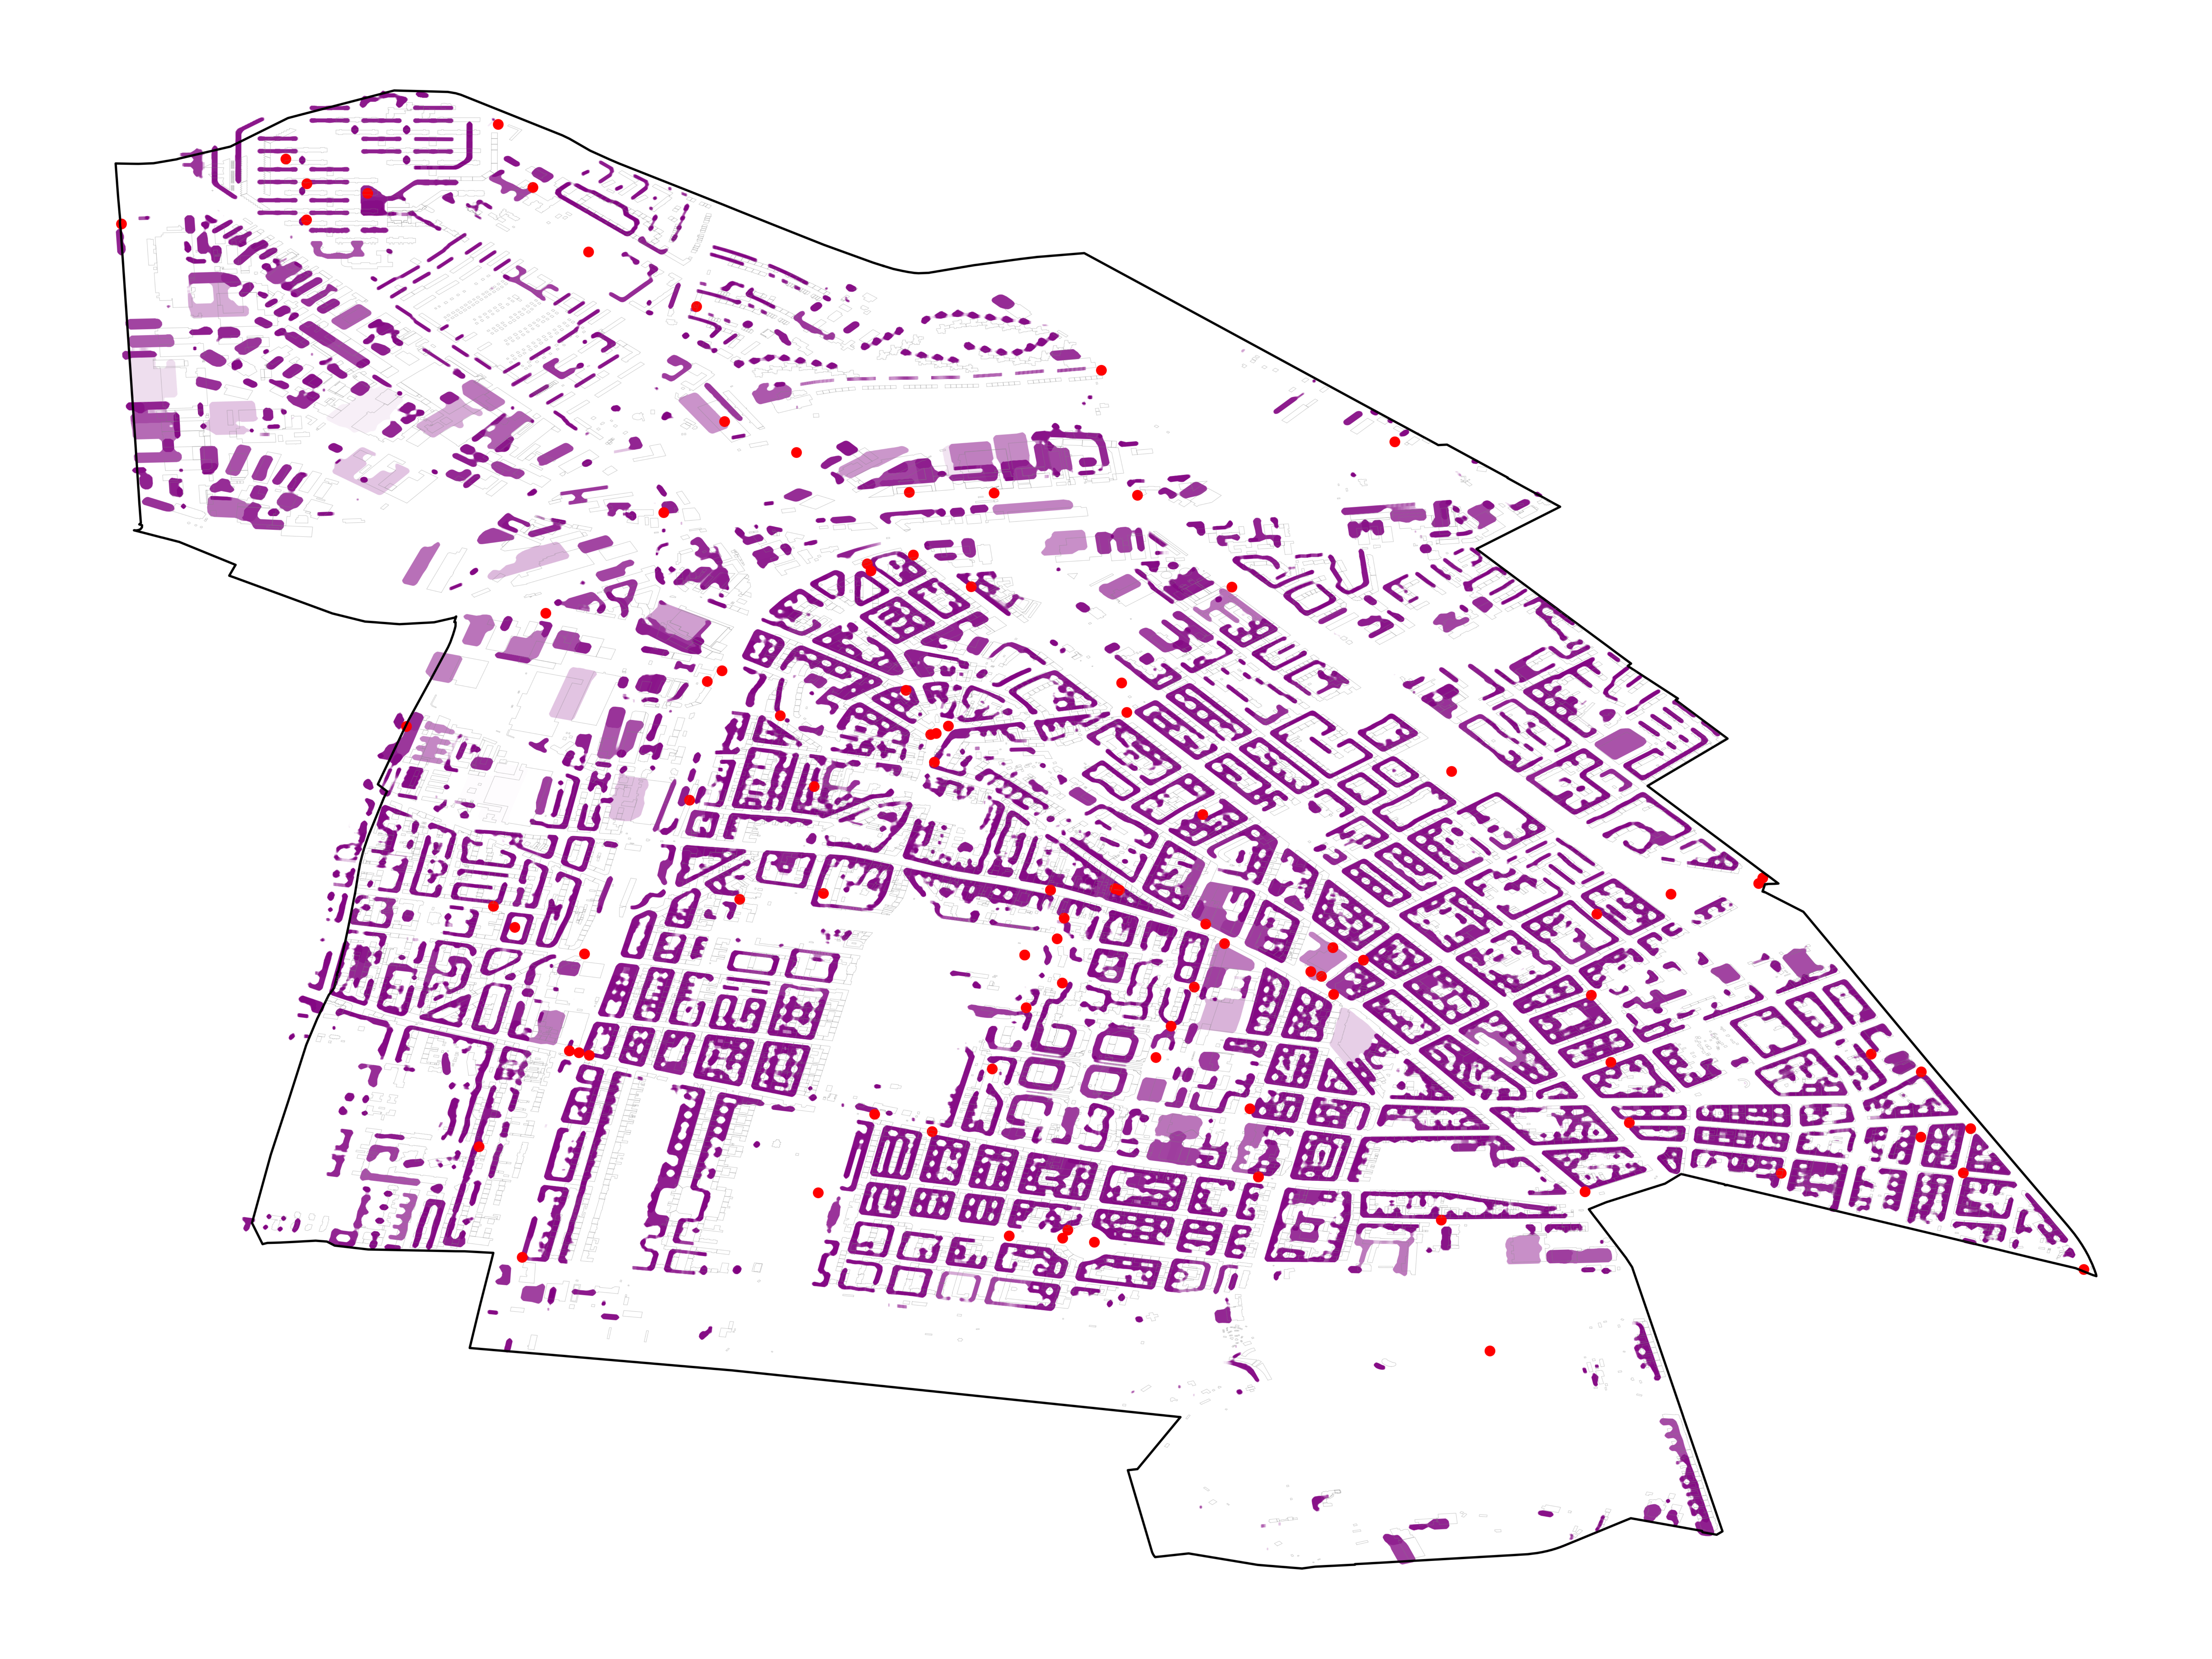
\includegraphics[width=0.5\textwidth]{figures/Adri/smaller_land_usage_with_crimes.png}& 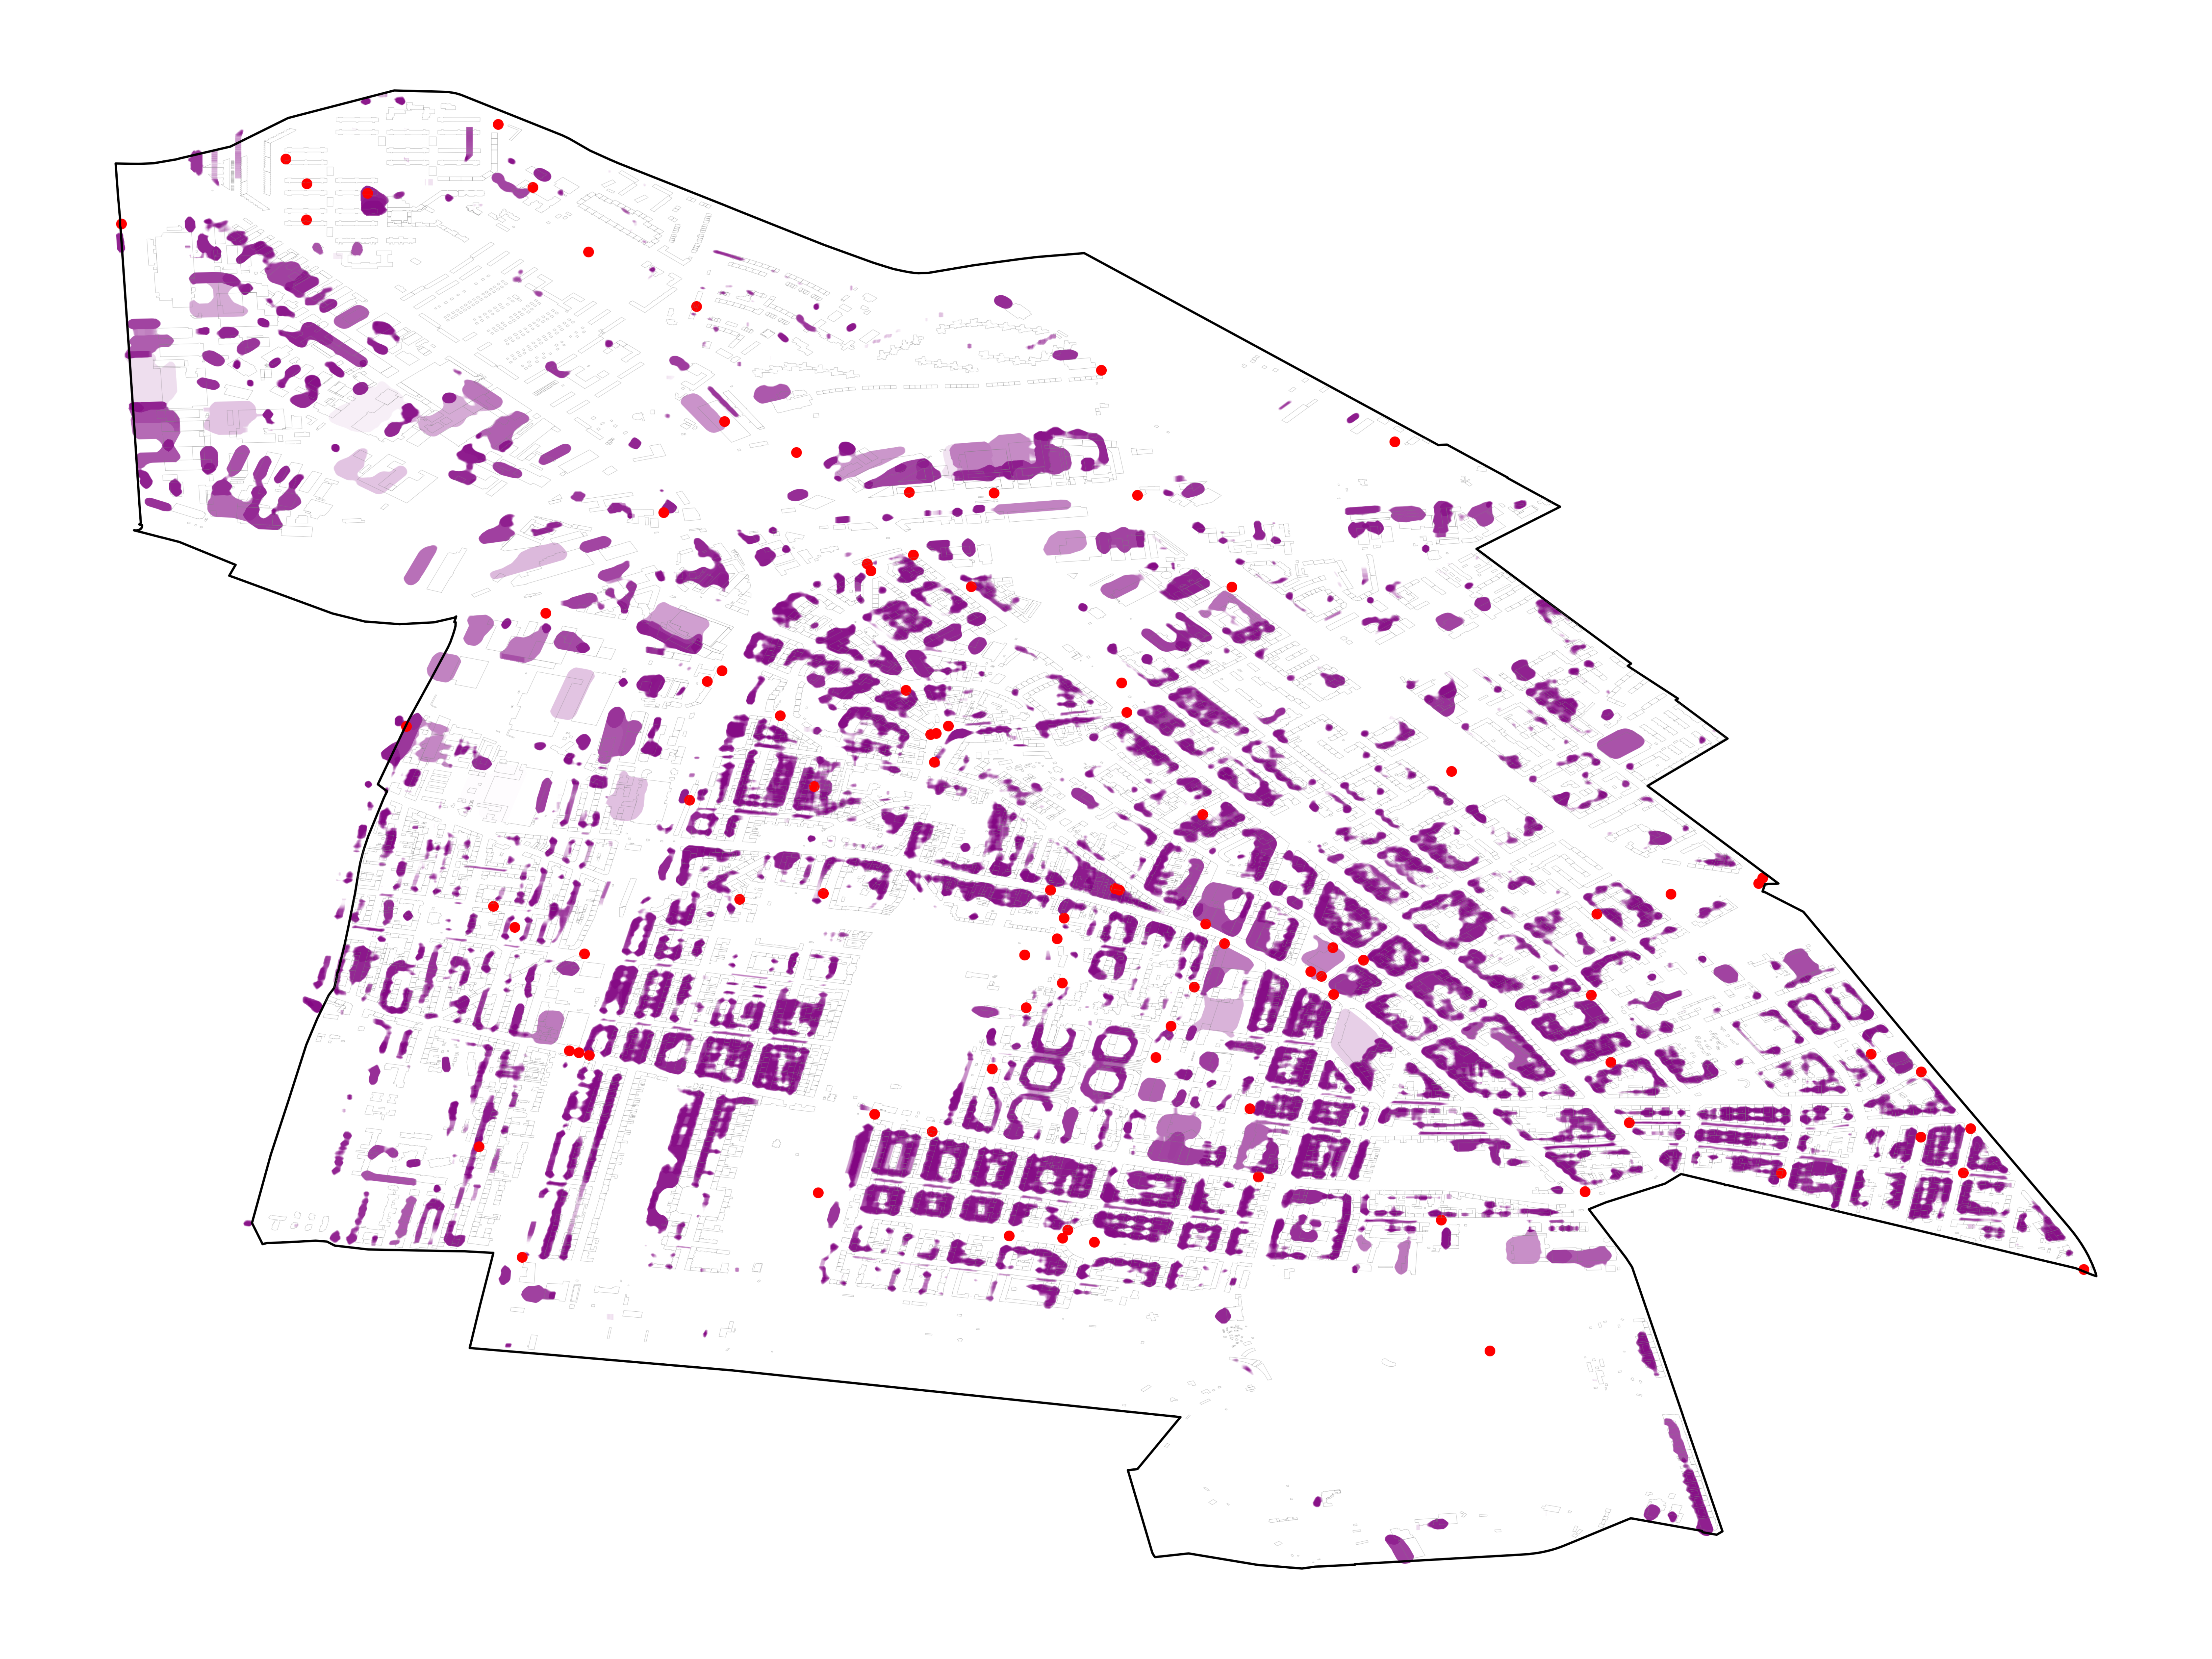
\includegraphics[width=0.5\textwidth]{figures/Adri/2land_usage.png}\\
         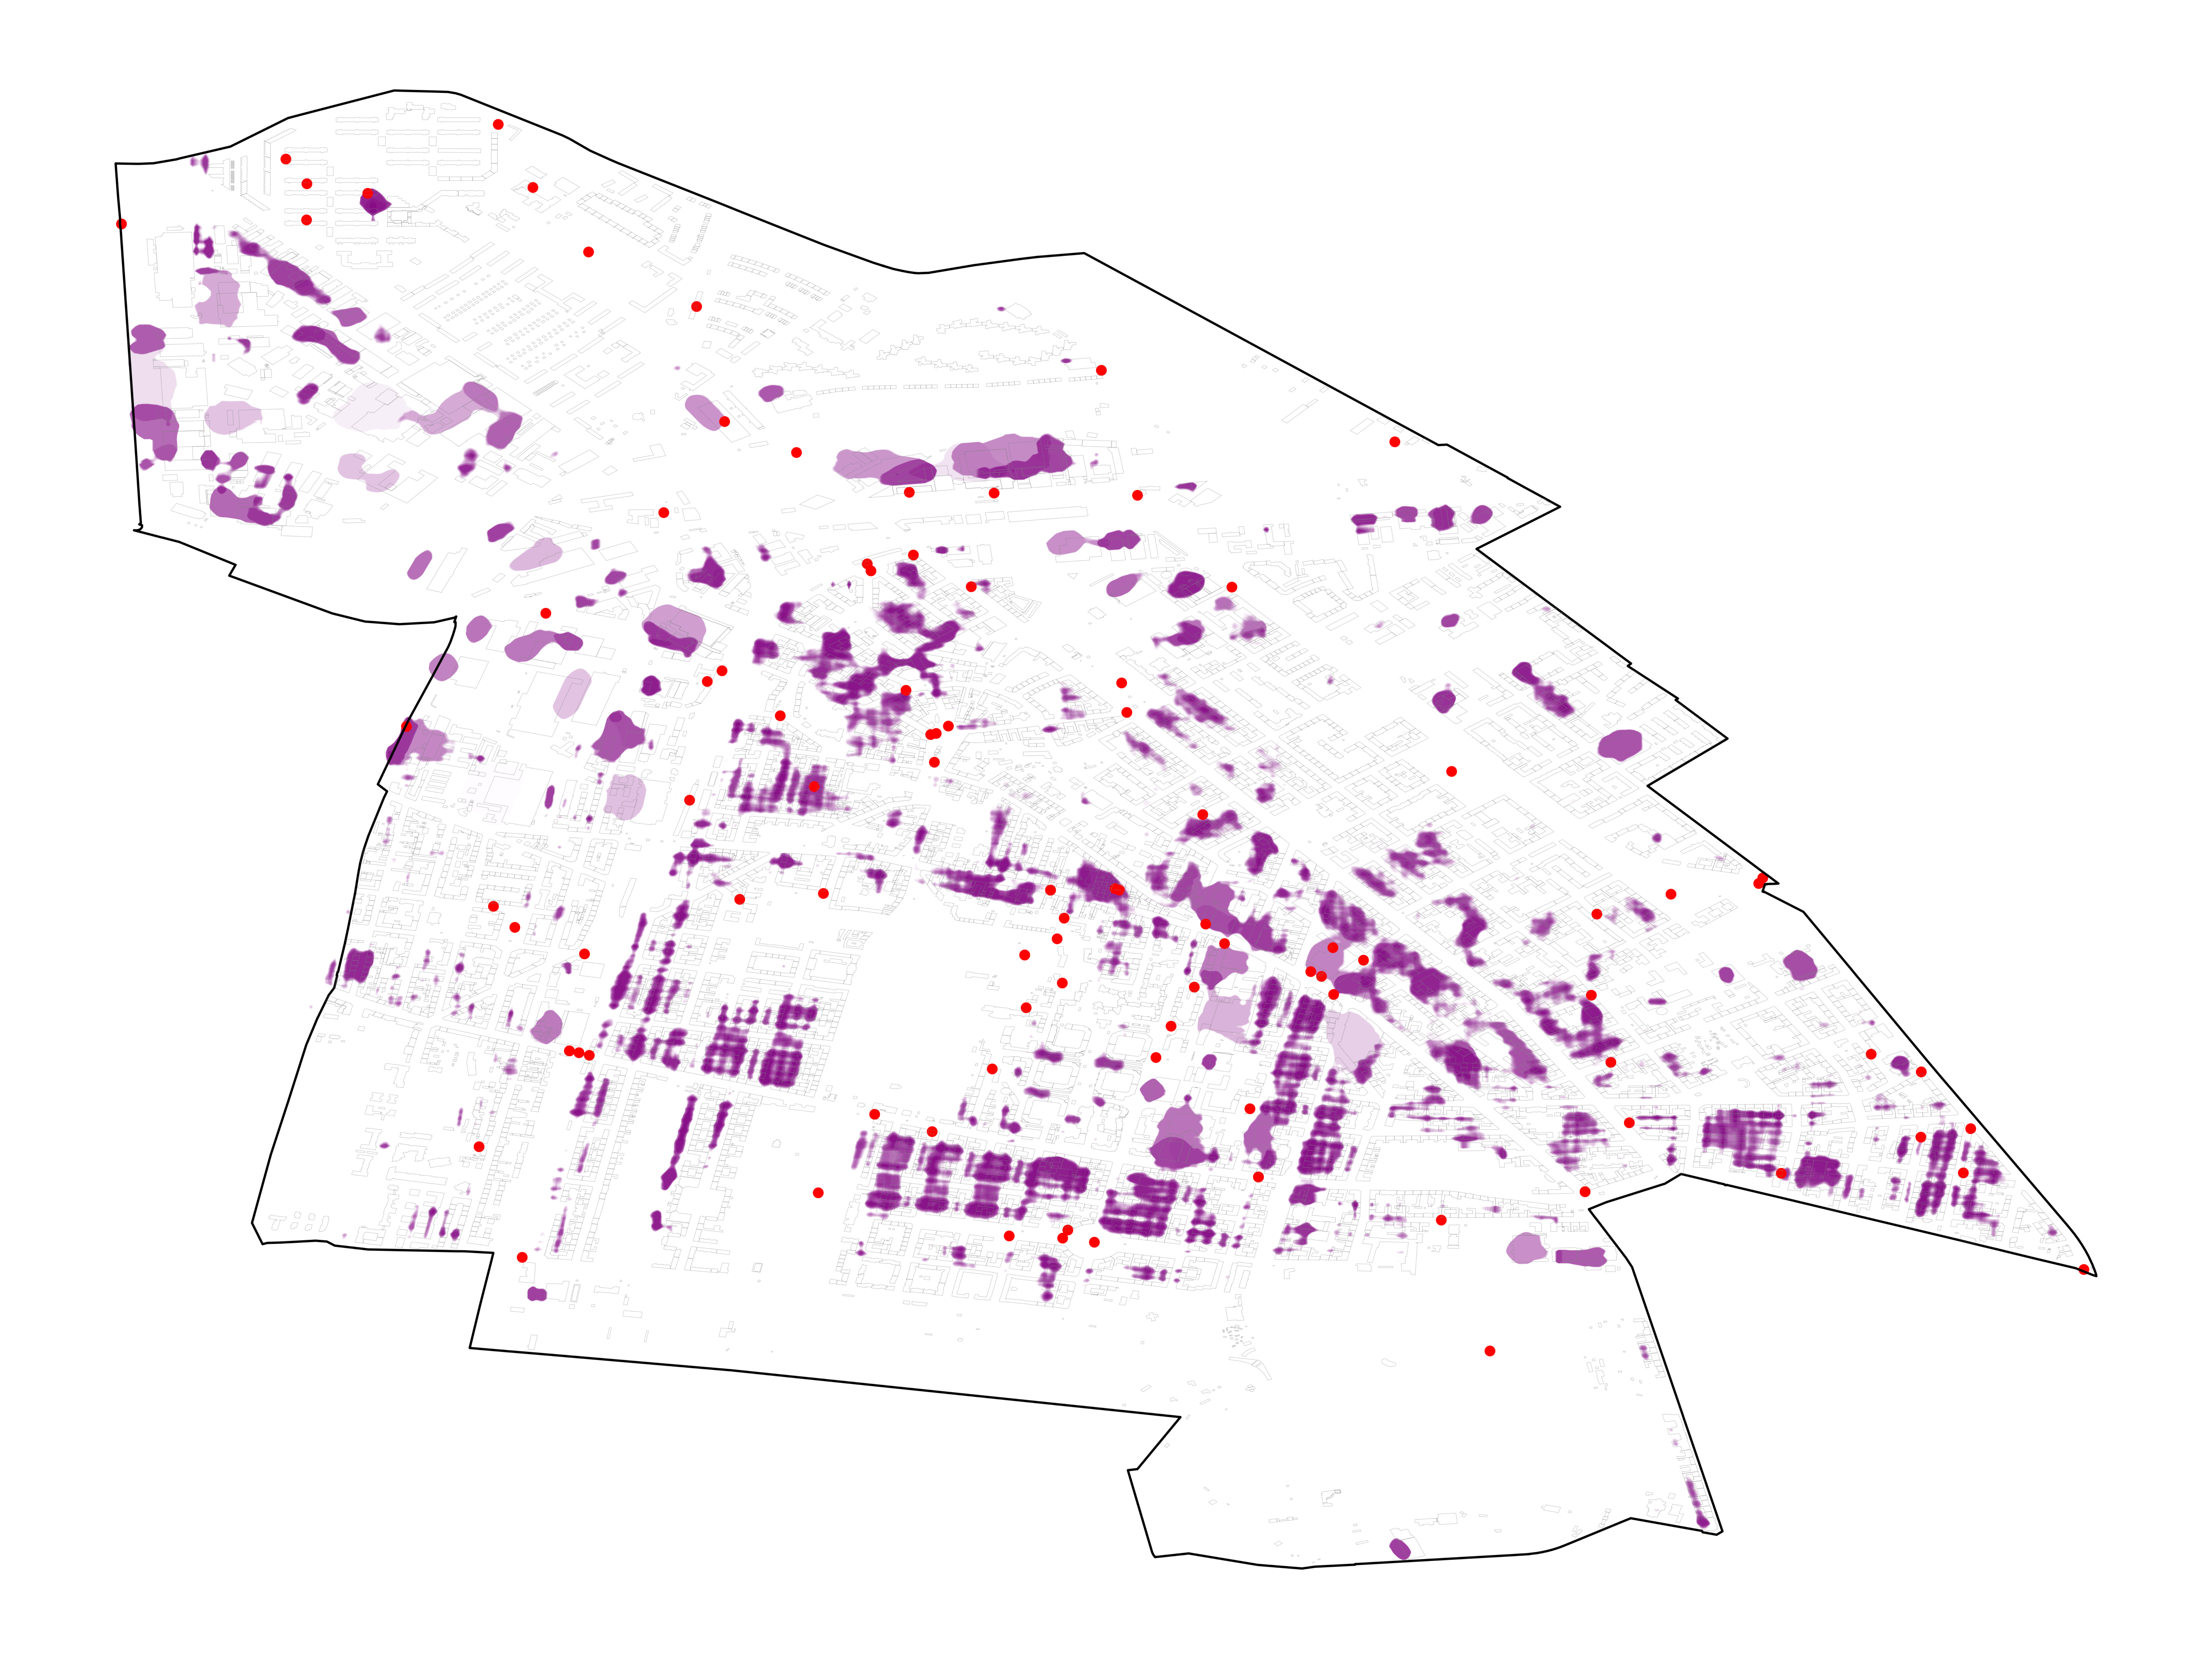
\includegraphics[width=0.5\textwidth]{figures/Adri/3land_usage.png}& 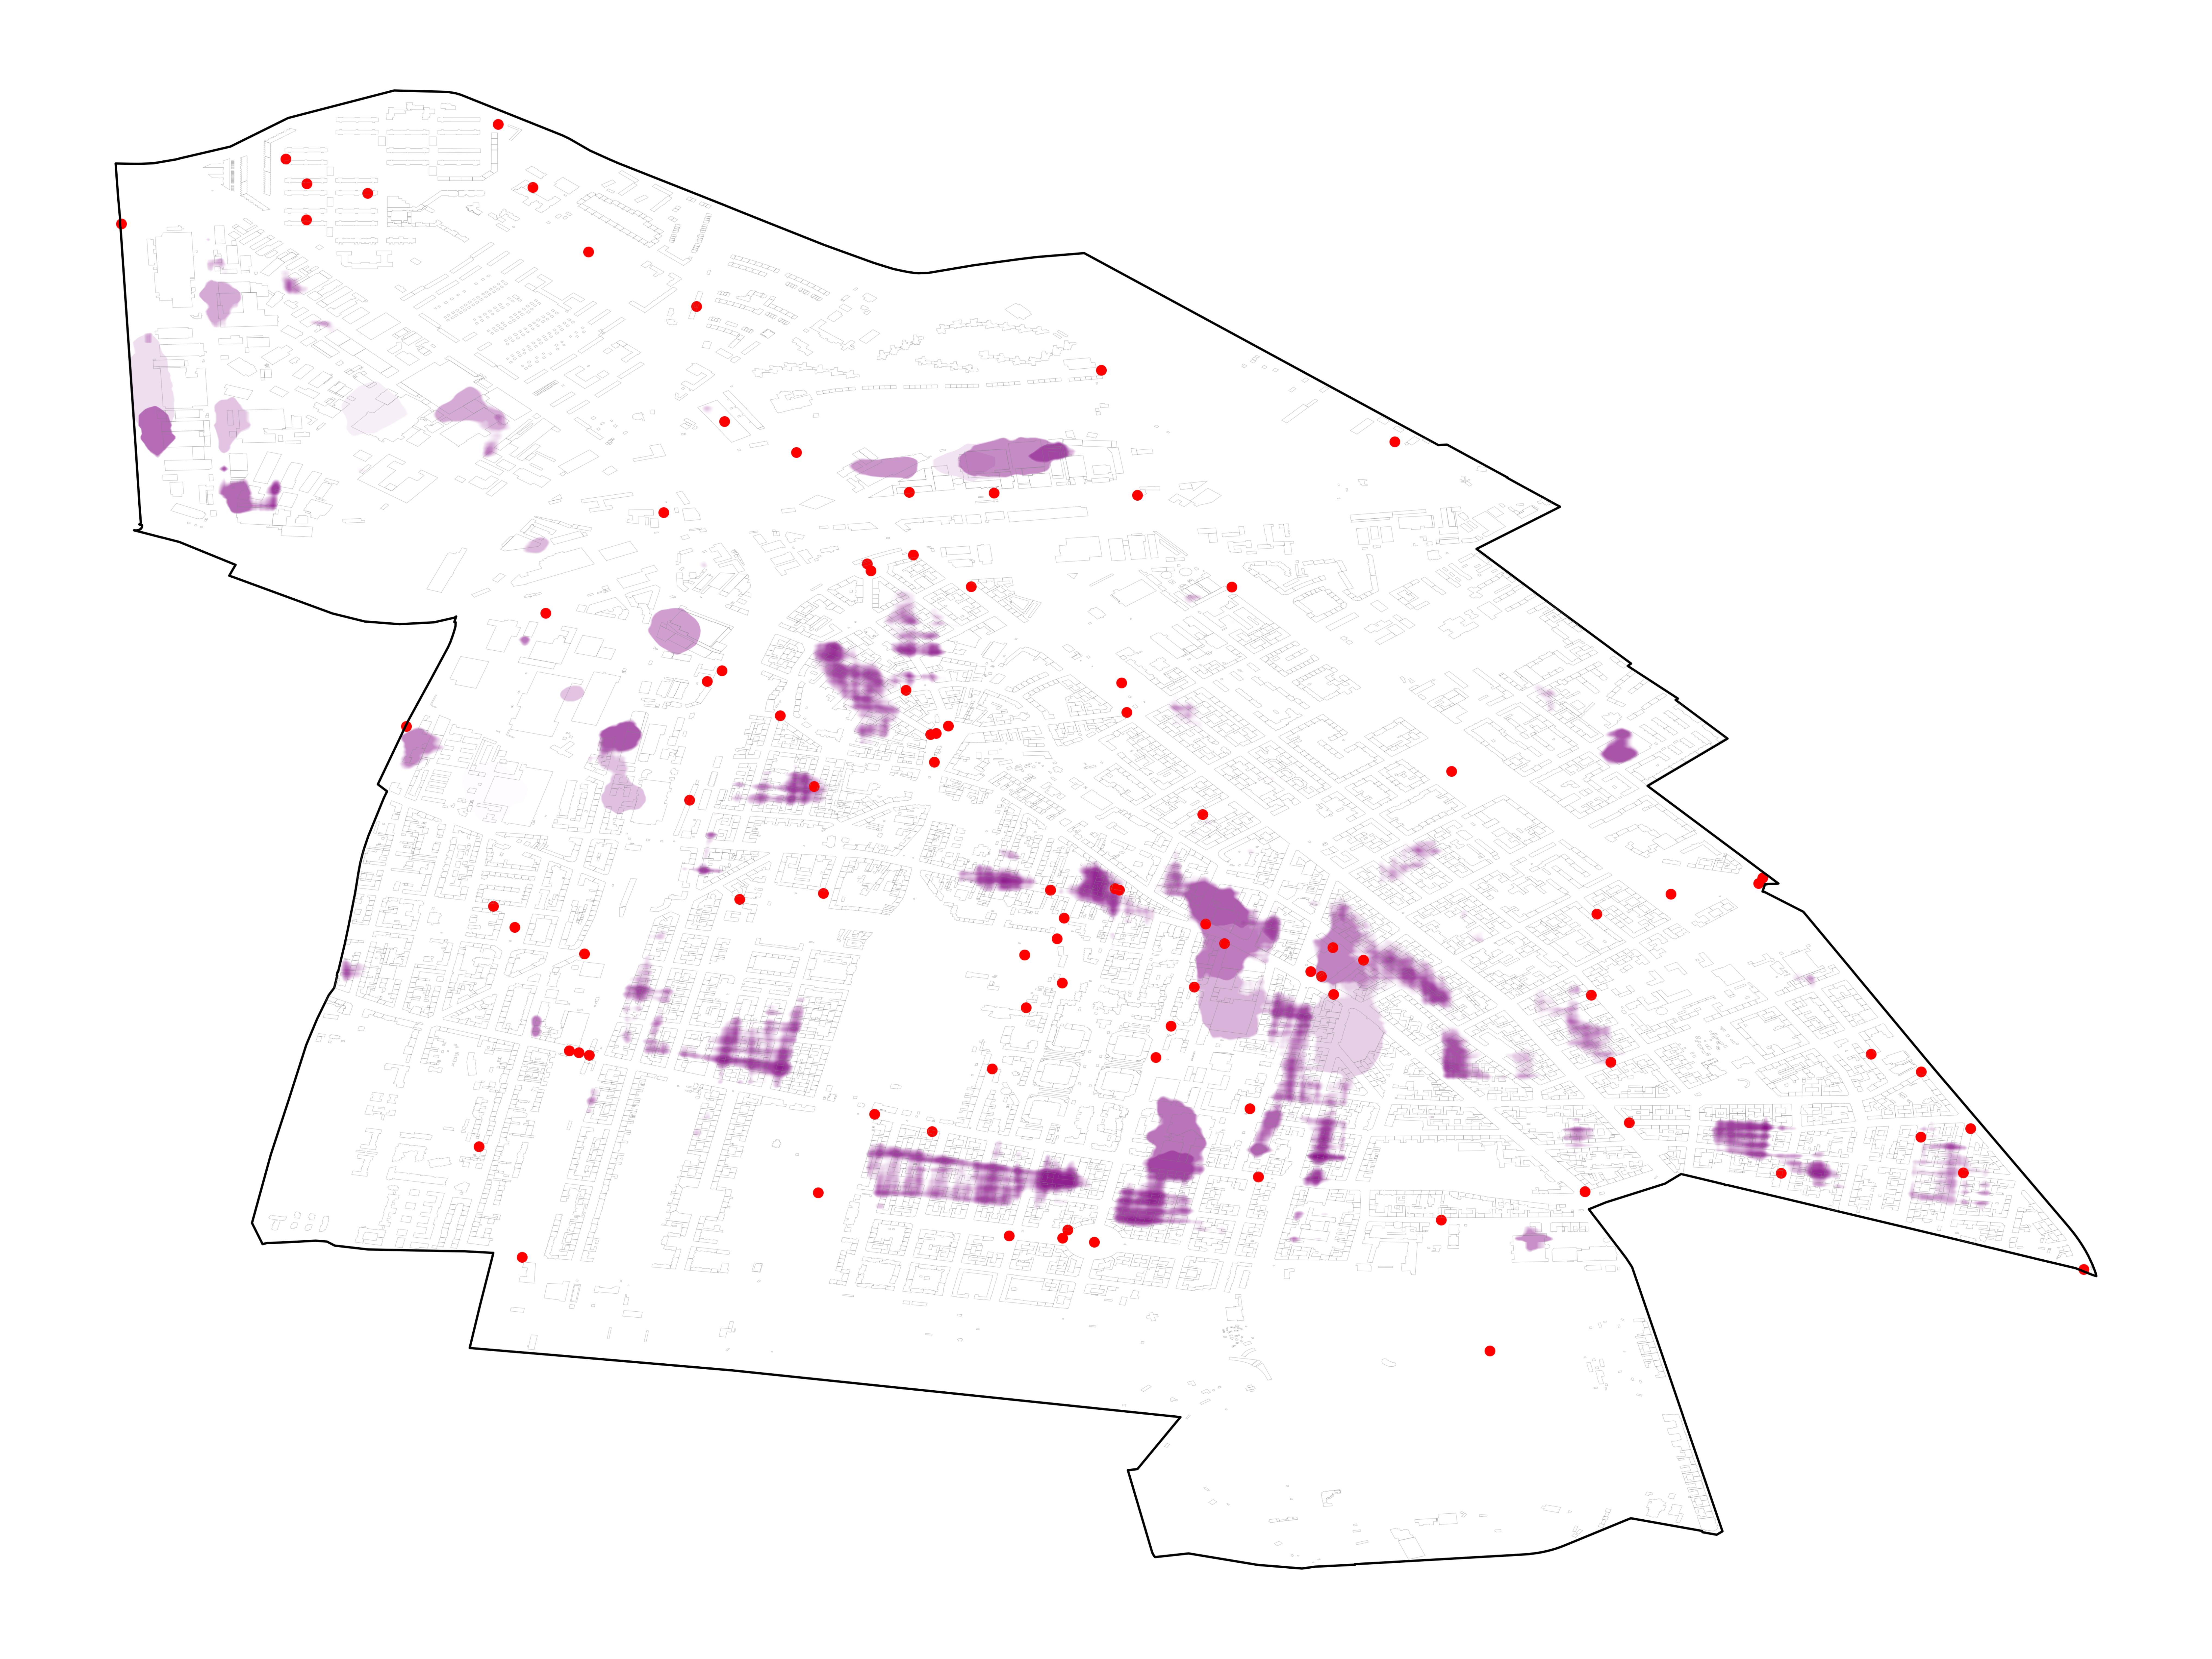
\includegraphics[width=0.5\textwidth]{figures/Adri/4land_usage.png}
    \end{tabular}
    \caption{Land usage analysis at four different scales: (top left) smallest scale with detailed land usage and crime locations, (top right) small scale, (bottom left) medium scale, and (bottom right) largest scale. Darker regions indicate areas with higher median land usage within each kernel. This multi-scale approach helps identify patterns and relationships between land use and crime rates.}
    \label{fig:landusage}
\end{figure}

\subsection{Lighting}
To analyze the distribution and coverage of street lighting, we employed a Voronoi diagram using the locations of all traffic lights in the city. This method partitions the urban area into regions, each centered around a single traffic light. The size and darkness of each region in the Voronoi diagram indicate the extent of the area served by a single traffic light. Larger and darker regions represent areas with fewer traffic lights, potentially highlighting zones with inadequate lighting coverage. This analysis is essential for identifying poorly lit areas that may require additional lighting to enhance safety and visibility for pedestrians and drivers.

\begin{figure}
\centering
\includegraphics[width=0.8\textwidth]{figures/Adri/lighting_voronoi.png}
\caption{Voronoi diagram of street lighting. The greater (and darker) the area, the larger the region covered by a single traffic light, indicating zones with potentially insufficient lighting.}
\label{fig
}
\end{figure}

\subsection{Corners}
In this section, we analyze the closure angles of street corners, as sharper angles can pose safety threats. Acute angles at intersections can limit visibility for both pedestrians and drivers, increasing the risk of accidents and crime. By identifying and mapping these angles, we can pinpoint hazardous intersections that may require redesign for improved safety and visibility.

\begin{figure}
\centering
\begin{tabular}{cc}
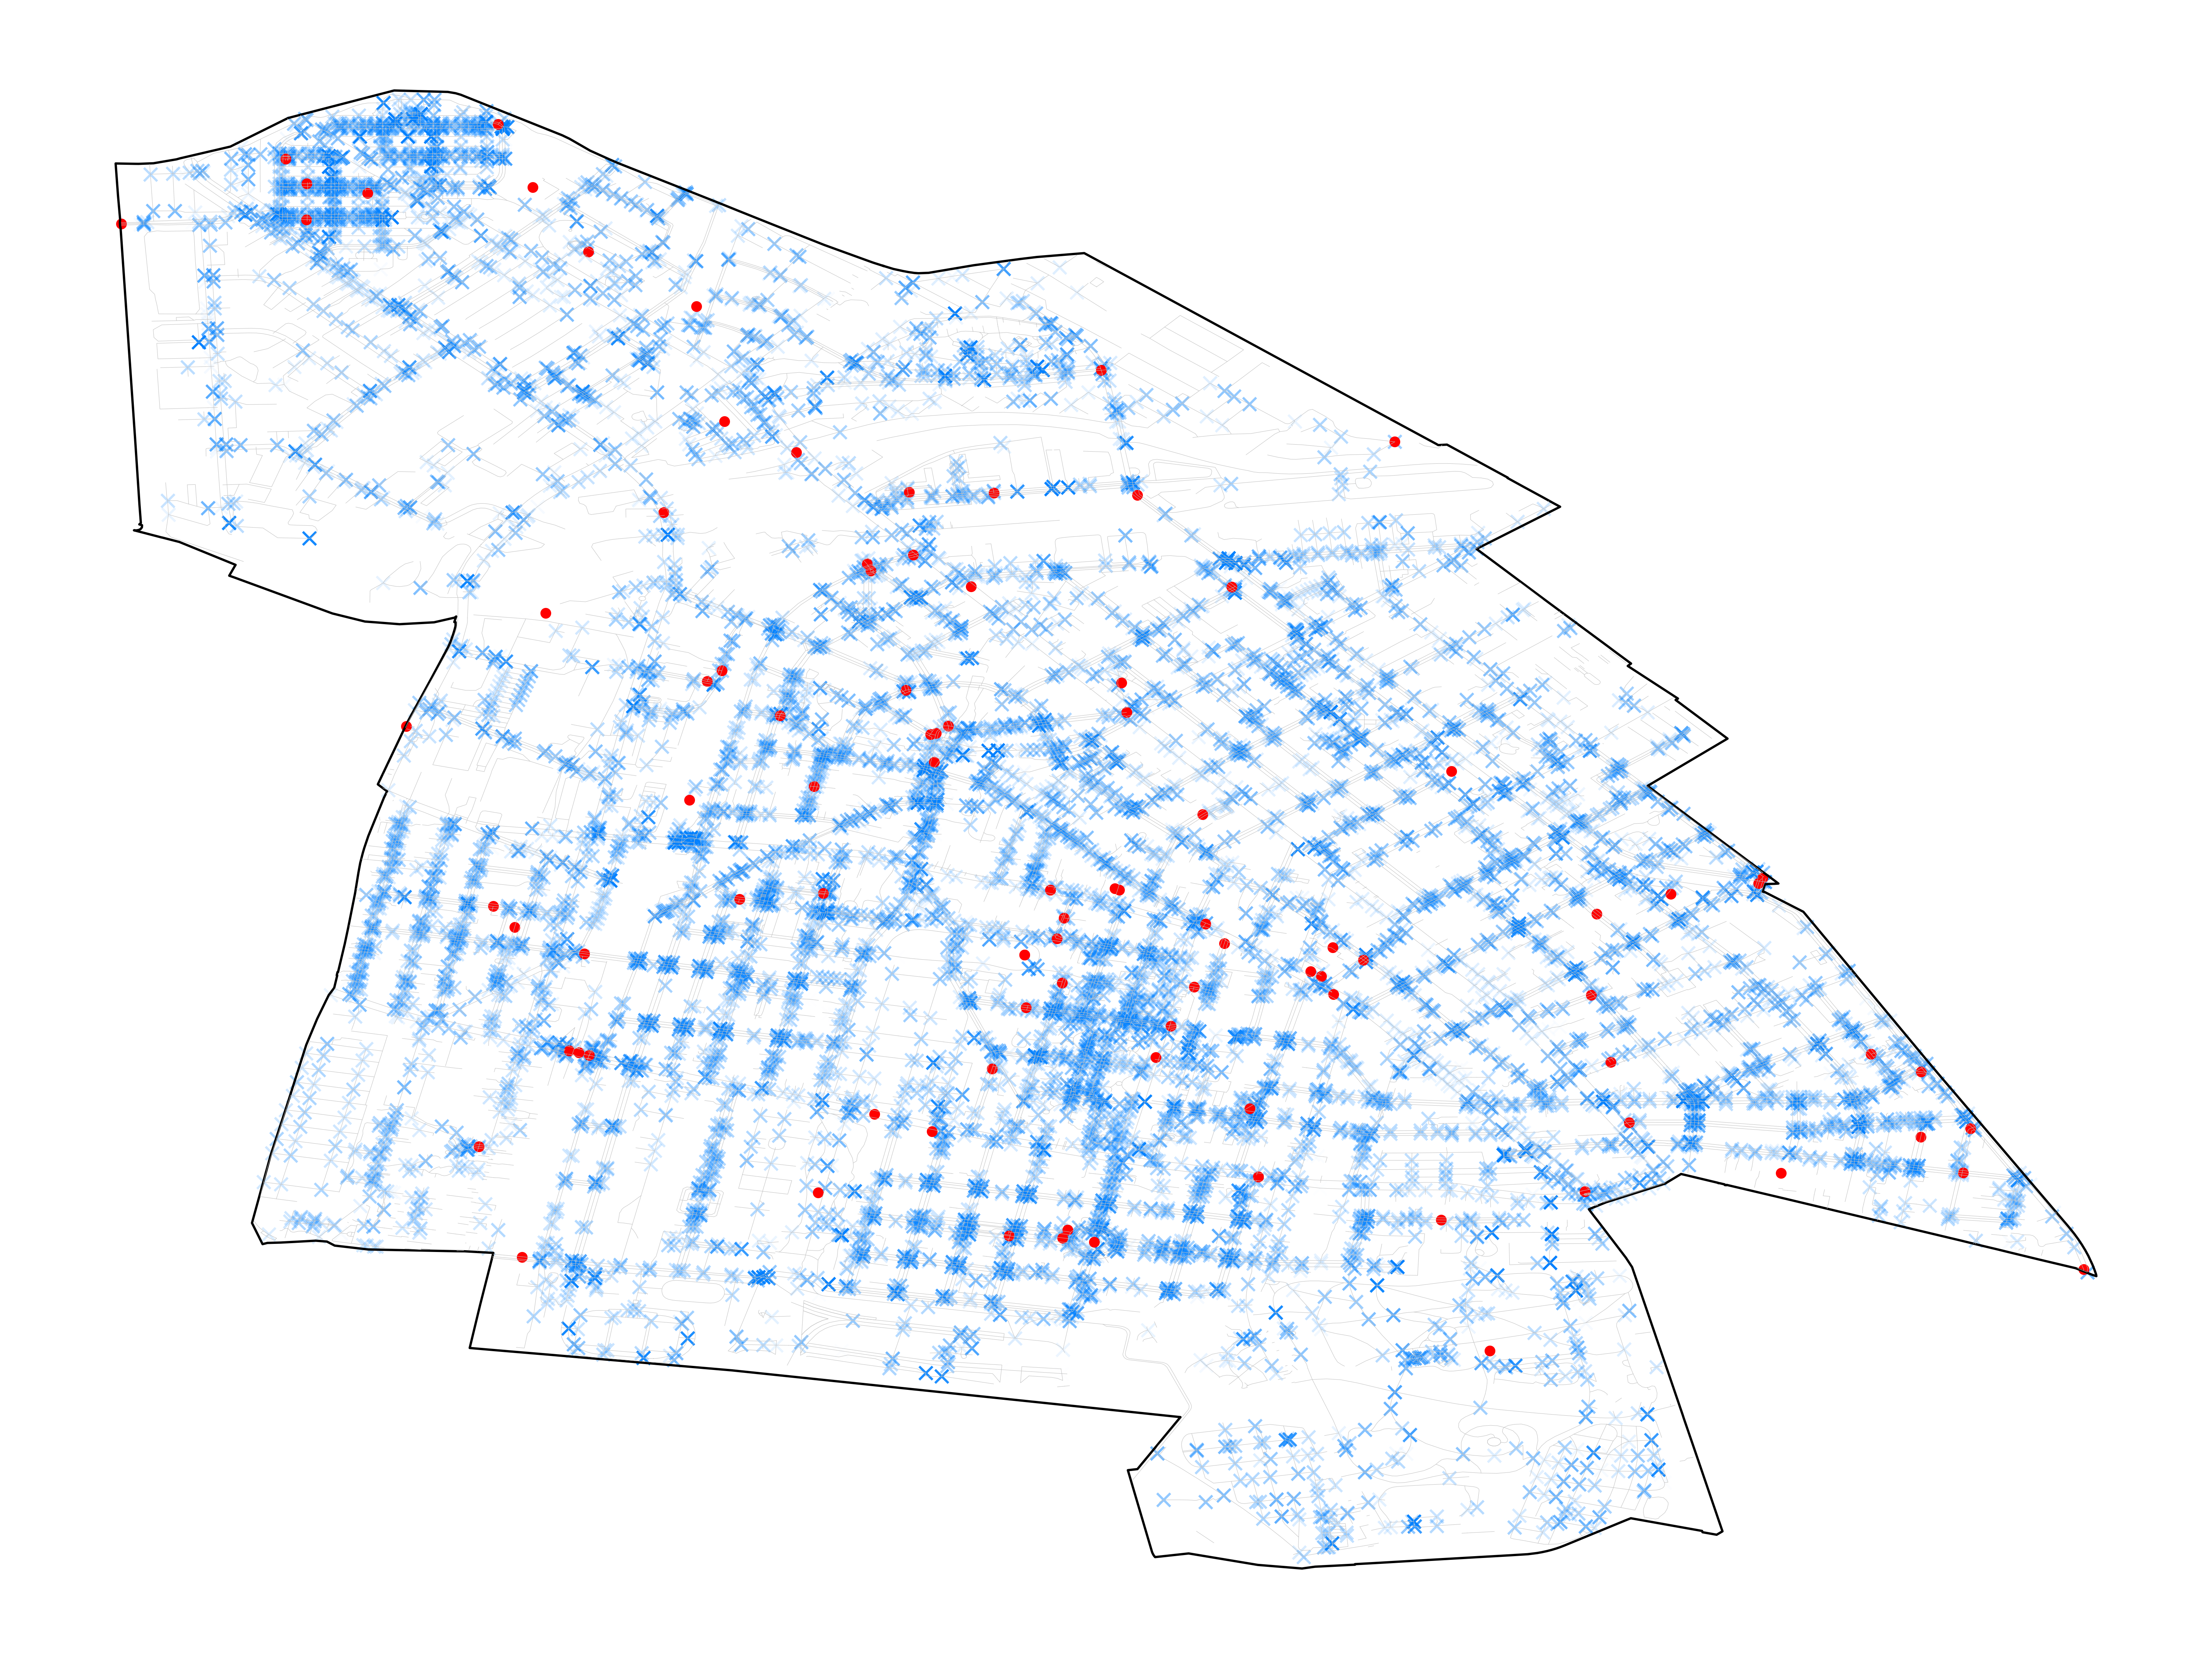
\includegraphics[width=0.5\textwidth]{figures/Adri/corners_ugly.png}& \includegraphics[width=0.5\textwidth]{figures/Adri/corners_nougly.png}
\end{tabular}
\caption{Analysis of street corner angles highlighting corners with acute angles that may pose safety risks.}
\label{fig
}
\end{figure}
